\documentclass[handout]{beamer}
\usetheme{Boadilla}
\usepackage{graphicx}

\title[Intermediation Frictions]{Intermediation Frictions in Incomplete Markets}
\subtitle{ECON 810A - Project}
\author{Alex von Hafften}
\institute{UW-Madison}

\begin{document}

\begin{frame}
\titlepage
\end{frame}

\begin{frame}
\frametitle{Secondary Treasury Market in COVID-19 Crisis}
\begin{itemize}[<+->]
\item The U.S. Treasury market - widely considered the world's deepest and most liquid financial market - is intermediated by large U.S. banks acting as broker-dealers.
\bigskip
\item In March 2020, concerns about COVID-19 prompted many large investors (e.g., hedge funds and foreign governments) to liquidate their holdings of Treasuries.
\bigskip
\item Intermediaries in the secondary market for U.S. Treasuries were overwhelmed (Duffie 2020).
\bigskip
\begin{itemize}[<+->]
\item Yield rose sharply.
\item Space on the balance sheet of broker-dealers for warehousing additional trades diminished.
\item Bid-offer spreads widened.
\item Settlement failures increased.
\end{itemize}
\bigskip
\item Aggressive intervention by the Fed restored market liquidity.
\end{itemize}
\end{frame}



\begin{frame}
\frametitle{Sources of Intermediation Frictions in Treasury Market}
\begin{itemize}[<+->]
\item This episode raised questions about the functioning of the secondary Treasury market, doubts about the safe-haven status of Treasuries, and calls for reform.
\bigskip
\item The growth in U.S. government debt outstanding may have outstripped the ability of broker-dealers to effective intermediate the secondary Treasury market.
\bigskip
\item Broker-dealers pointed to post-financial-crisis bank regulatory reform - in particular, the Supplementary Leverage Ratio requirement - as the source of the disruption.
\bigskip
\item \textbf{Research Question:} How does the intermediation of illiquid assets affect portfolio choice?
\end{itemize}
\end{frame}



\begin{frame}
\frametitle{Multiple Assets}
\begin{itemize}[<+->]
\item To explore this question, I turned to Bewley-style models with multiple assets.
\bigskip
\item In the baseline Bewley model (and models covered in ECON 810A), household can only invest in one-period risk-free bonds.
\bigskip
\item In reality, households invest in many assets, including cash, real estate, stocks, bonds, etc.
\bigskip
\item Optimal portfolio choices change with wealth and age (Brandsas 2020).
\bigskip
\item The curse of dimensionality quickly hampers rich portfolio choice problems in Bewley-style model.
\end{itemize}
\end{frame}





\begin{frame}
\frametitle{Literature Review - Kaplan and Violante (2014)}


\begin{itemize}[<+->]
\item Empirical literature finds that households spend about 25 percent of tax rebates on consumption immediately inconsistent with prediction from single-asset Bewley.
\bigskip
\item Build a Bewley-style model with two assets: low return liquid asset and high return illiquid asset.
\bigskip
\item HHs must pay fixed cost to adjust illiquid asset holding.
\bigskip
\item Many HHs are optimally ``wealthy hand-to-mouth" (i.e., hold very little liquid assets despite sizable amount of illiquid assets).
\bigskip
\item Wealthy hand-to-mouth HHs have high MPC and rationalize empirical motivation.
\end{itemize}

\end{frame}



\begin{frame}
\frametitle{Literature Review - Rios-Rull and Sanchez-Marcos (2008)}

\begin{itemize}[<+->]
\item Build a Bewley-style model with financial assets and nonfinancial assets.
\bigskip
\item Financial assets are perfectly divisible and costless to buy or sell.
\bigskip
\item Nonfinancial assets are bulky, indivisible, and have transaction costs.
\bigskip
\item Label the nonfinancial assets as ``houses".
\bigskip
\item Find reasonable lifecycle pattern: HHs accumulate some financial assets for downpayment, then buy a small house, then buy a large house.
\bigskip
\item HHs pay a fixed cost to trade their house.
\end{itemize}

\end{frame}




\begin{frame}
\frametitle{Approach}

\begin{itemize}[<+->]
\item Similar to Kaplan and Violante (2014) and Rios-Rull and Sanchez-Marcos (2008), I use two assets. 
\bigskip

\begin{itemize}[<+->]
\item Here, cash and a long-term bond with stochastic maturity.
\end{itemize}

\bigskip
\item Instead of second asset coming from fixed transaction cost, I use random search for intermediary (i.e. broker-dealer).
\end{itemize}

\end{frame}






\begin{frame}
\frametitle{Environment}

\begin{itemize}[<+->]

\item Two agents: 
\begin{itemize}[<+->]

\item Households.
\item Intermediaries.

\end{itemize}

\bigskip

\item Two assets:

\begin{itemize}[<+->]

\item Cash/consumption good without no return.
\item Long-term illiquid bonds with return $r$. 
\item Fraction $\delta \in (0, 1)$ of long-term bonds mature into cash each period. 

\end{itemize}

\bigskip

\item Households randomly search for intermediaries:

\begin{itemize}[<+->]

\item If an household and an intermediary meet, the household can sell long-term bonds.
\item Nash bargain over price with $\theta \in (0, 1)$ being the bargaining power of the household. 
\item Households can always buy long-term bonds (i.e. ``on-the-run" Treasuries), but can only sell them through an intermediary (e.g. ``off-the-run" Treasuries).

\end{itemize}

\end{itemize}

\end{frame}



\begin{frame}
\frametitle{Model Timing}

\begin{enumerate}[<+->]

\item Exogenous labor income is drawn.
\item Long-term bonds return $r$.
\item Households and intermediaries meet.
\item Consumption good is eaten.
\item Households and intermediaries bargain and trade.
\item Value functions are evaluated.

\end{enumerate}

\end{frame}





\begin{frame}
\frametitle{Intermediaries}

\begin{itemize}[<+->]

\item Intermediaries are infinitely lived and risk-neutral.
\item Discount factor $\beta_I$.
\item They have ``deep pockets".
\item They consume long-term bonds as they mature.
\item Their value for buying $b$ long-term bonds from a HH:

\begin{align*}
W(b) 
&= \underbrace{\beta_I\delta b}_{\text{consumption one period after trade}} + \underbrace{\beta_I^2(1-\delta)\delta b}_{\text{consumption two period after trade}} \\
&+ \underbrace{\beta_I^3(1-\delta)^2\delta b}_{\text{consumption three periods after trade}} + ...\\\\
&= \frac{\beta_I\delta b }{1 - \beta_I (1-\delta)}
\end{align*}

\end{itemize}

\end{frame}





\begin{frame}
\frametitle{Households}

\begin{itemize}[<+->]

\item Live for $T$ periods.
\item Risk averse.
\item Discount factor $\beta$.
\item Exogenous Markov process for labor earnings $y$.
\item Make consumption-savings choice with zero borrowing limit.
\item Hold cash $a$.
\item Hold long-term illiquid bonds $b$.
\item Meet an intermediaries with probability $\gamma$ and can liquidate fraction $\ell$ of their long-term illiquid bonds.
\item The HHs value function is:

$$
V_t(y, a, b) \equiv \gamma \underbrace{V^M_{t}(y, a, b)}_{\text{value if matched}} + (1-\gamma) \underbrace{V^U_{t}(y, a, b)}_{\text{value if matched}}
$$

\end{itemize}

\end{frame}






\begin{frame}
\frametitle{Unmatched Households Value Function}

\begin{itemize}[<+->]

\item A HH that is not matched with an intermediary choose consumption $c$, cash tomorrow $a'$, and purchase new long-term bonds $\tilde{b}'$ to maximize utility:

\begin{align*}
V_{t}^U(y, a, b) 
= \max_{c, a', \tilde{b}'} 
\Bigg\{ 
\underbrace{u(c)}_{\text{instantaneous value}} 
&+ \underbrace{\beta E[V_{t+1}(y', a', b')]}_{\text{continuation value }} \Bigg\}
\end{align*}

subject to

\begin{align*}
c + a' + \underbrace{\tilde{b}'}_{\text{new LT bonds}} &= y + a + \underbrace{\delta b (1 + r)}_{\text{matured LT bonds}} \\ 
b' &= \underbrace{\tilde{b}'}_{\text{new LT bonds}} + \underbrace{(1-\delta)b(1+r)}_{\text{unmatured LT bonds}}\\
a', \tilde{b}' &\ge 0
\end{align*}

\end{itemize}

\end{frame}




\begin{frame}
\frametitle{Matched Households Value Function}

\begin{itemize}[<+->]

\item A HH that is matched with an intermediary can either buy LT bonds (same problem as unmatched) or sell LT bonds:

\begin{align*}
&V_{t}^M(y, a, b) 
= \max
\Bigg\{ 
\underbrace{ V_t^U(y, a, b)}_{\text{buying LT bonds}},\\&\underbrace{ \max_{c, a', \ell} 
\Bigg\{ u(c) + \beta E[V_{t+1}(y', a'+\overbrace{P(\ell (1-\delta)b(1+r))}^{\text{proceeds from selling LT bonds}}, b')] \Bigg\}}_{\text{selling LT bonds }} \Bigg\}
\end{align*}

subject to

\begin{align*}
c + a' &= y + a + \delta b (1 + r)\\
b' &= \underbrace{(1-\ell)(1-\delta)b(1+r)}_{\text{unsold, unmatured LT bonds}}, \; \; \; a' \ge 0, \ell \in [0, 1]
\end{align*}

\end{itemize}

\end{frame}









\begin{frame}
\frametitle{Nash Bargaining}

\begin{itemize}[<+->]

\item The matched household has $\hat{b}' \equiv \ell(1-\delta)b(1+r)$ LT bonds to sell.

\bigskip

\item The value to the intermediary is $W(\hat{b}') - P$.

\bigskip

\item The outside option for the intermediary is zero. 

\bigskip

\item The value to the household is $\beta E[V_{t+1}(y', a' + P, b')]$.

\bigskip

\item The outside option for the household is the unmatched value function: $\beta E[V_{t+1}(y', a', b' + \hat{b}')]$.

\end{itemize}

\end{frame}


\begin{frame}
\frametitle{Nash Bargaining (con't)}

\begin{itemize}[<+->]

\item Nash bargaining solves:

\begin{align*}
\max_{P} \Bigg[\underbrace{\beta E[V_{t+1}(y', a' + P, b') - \beta E[V_{t+1}(y', a', b' + \hat{b}')]}_{\text{surplus of HH}}\Bigg]^\theta \\
\times \Bigg[\underbrace{ W(\hat{b}') - P}_{\text{surplus of intermediary}}\Bigg]^{1-\theta}
\end{align*}

\hyperlink{nb_foc}{ \beamerbutton{FOC}}

\end{itemize}

\end{frame}



\begin{frame}
\frametitle{Nash Bargaining (con't)}

\begin{align*}
&\theta E[V_{a,t+1}(y', a' + P, b')] \Bigg[ W(\hat{b}') - P\Bigg]\\
&- (1-\theta)\Bigg[ E[V_{t+1}(y', a' + P, b') - E[V_{t+1}(y', a', b' + \hat{b}')]\Bigg] = 0
\end{align*}

\bigskip

We can solve this pricing condition numerically by:

\begin{itemize}[<+->]
\item Numerically calculating $E[V_{a,t+1}(y', a' + P, b')]$.
\item Using root solver.
\end{itemize}

\end{frame}







\begin{frame}
\frametitle{Computational Strategy}
\begin{itemize}[<+->]
\item Start at period $T$, where households eat all labor earnings, cash, and matured long-term bonds. There's no $T+1$ period, so matched HHs do not liquidate any LT bonds.
\bigskip
\item For any period $t$, 
\begin{itemize}[<+->]
\item Solve unmatched HH problem.
\item Solve matched HH problem conditional on selling LT bonds. Guess $\ell$ and $a'$, solve price condition (with root solver) for $P$, evaluate value function, and choose optimum.
\item Matched HH problem solution is max of unmatched solution and matched solution conditional on selling.
\end{itemize}
\bigskip
\item Use linear interpolations due to two continuous state variables. 
\bigskip
\item Coarse grid for solving the model; finer grid for simulating the model.
\end{itemize}
\end{frame}





\begin{frame}
\frametitle{Calibration}

\begin{itemize}[<+->]

\item Average maturity of outstanding U.S. Treasury is 70 months, so $\delta = 0.17143$. \hyperlink{delta}{ \beamerbutton{more}}
\item CRRA utility with coefficient of relative risk aversion equal to 2.
\item Annual frequency.
\item Two state Markov earnings process with $y_e = 1.0$ and $y_u = 0.5$ with $\pi_{ee} = 0.9$ and $\pi_{uu} = 0.5$ to match employment rate and employment duration.
\item $T = 30$.
\item $\beta = 0.99$
\item $\theta = 0.5$
\item $r = 0.1$
\bigskip

\end{itemize}

\end{frame}


\begin{frame}
\frametitle{Policy Experiments changing Intermediation Frictions}

\begin{center}
\begin{tabular}{ l | r r r }
& Baseline & Policy Experiment \#1 & Policy Experiment \#2\\ 
\hline 
$\beta_I$ & 0.99 & 0.95 & 0.99 \\
$\gamma$  & 0.2 & 0.2 & 0.1 \\ 
\end{tabular}
\end{center}

\bigskip


\begin{itemize}[<+->]
\item Policy Experiment \#1: Intermediaries are less patient $\implies$ consuming $b$ over time less $\implies$ price drops
\begin{align*}
\frac{\partial W(b)}{\partial \beta_I} &= \frac{\delta b }{[1 - \beta_I (1-\delta)]^2} > 0
\end{align*}
\bigskip
\item Policy Experiment \#2: HH is less likely to meet intermediate.
\end{itemize}


\end{frame}





\begin{frame}
\frametitle{Policy Experiment \#1}

\begin{center}
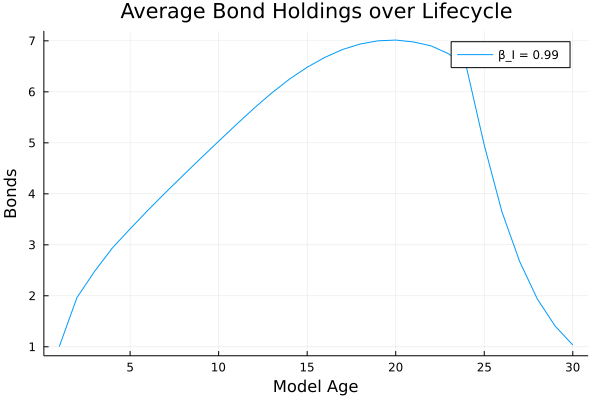
\includegraphics[scale = 0.5]{bond}
\end{center}

\end{frame}



\begin{frame}
\frametitle{Policy Experiment \#1}

\begin{center}
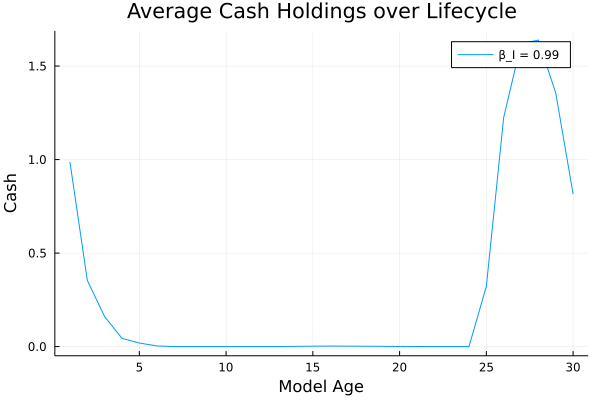
\includegraphics[scale = 0.5]{cash}
\end{center}

\end{frame}


\begin{frame}
\frametitle{Policy Experiment \#1}

\begin{center}
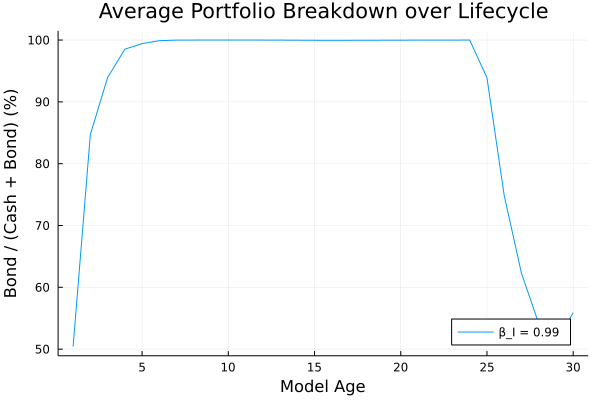
\includegraphics[scale = 0.5]{portfolio}
\end{center}

\end{frame}


\begin{frame}
\frametitle{Something is wrong here...}

\begin{center}
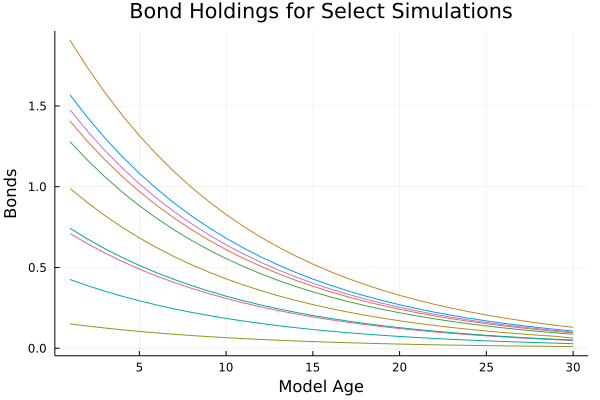
\includegraphics[scale = 0.5]{problem}
\end{center}

\end{frame}






\begin{frame}
\frametitle{References}
\scriptsize

Brandsas, Eirik (2020) ``Stock Market Participation and Exit: The Role of Homeownership," Working Paper.

\smallskip

Duffie, Darrell (2020) ``Still the World's Safe Haven? Redesigning the U.S. Treasury Market After the COVID-19 Crisis," Hutchins Center Working Paper \#62, June 2020.

\smallskip

Kaplan, Greg and Giovanni L. Violante (2014). ``A Model of the Consumption Response to Fiscal Stimulus Payments," Econometrica, Vol. 82, No. 4, July 2014, 1199-1239.

\smallskip

Rios-Rull, Jose-Victor and Virginia Sanchez-Marcos (2008). ``An Aggregate Economy with different Size Houses," Journal of European Economic Association, Vol. 6, No. 2/3, Proceedings of the Twenty-Second Annual Congress of the European Economic Association (Apr. - May, 2008), pp. 705-714

\end{frame}


\begin{frame}[label = nb_foc]
\frametitle{Nash Bargaining (con't)}

\begin{itemize}[<+->] 

\item First order condition:

\begin{align*}
\theta \Bigg[&\beta E[V_{t+1}(y', a' + P, b') - \beta E[V_{t+1}(y', a', b' + \hat{b}')]\Bigg]^{\theta-1} \\
&\times \beta E[V_{a,t+1}(y', a' + P, b')] \Bigg[ W(\hat{b}') - P\Bigg]^{1-\theta}\\
&= (1-\theta)\Bigg[ W(\hat{b}') - P\Bigg]^{-\theta}\\
&\times\Bigg[\beta E[V_{t+1}(y', a' + P, b') - \beta E[V_{t+1}(y', a', b' + \hat{b}')]\Bigg]^\theta
\end{align*}

\end{itemize}

\end{frame}





\begin{frame}[label = delta]
\frametitle{Calibration $\delta$}


Average maturity of LT bond is:

$$
\delta + 2(1-\delta)\delta + 3(1-\delta)^2 \delta + ... = \delta \sum_{t=1}^\infty  t (1-\delta)^{t-1}
$$

For average maturity of $70/12 \approx 5.833 \implies \delta \approx 0.17143$ 

\end{frame}





\end{document}

